\documentclass{article}

% Language setting
% Replace `english' with e.g. `spanish' to change the document language
\usepackage[italian]{babel}

% Set page size and margins
% Replace `letterpaper' with `a4paper' for UK/EU standard size
\usepackage[letterpaper,top=2cm,bottom=2cm,left=3cm,right=3cm,marginparwidth=1.75cm]{geometry}
  \usepackage{minted}
 \usepackage[dvipsnames]{xcolor}
\definecolor{lightGray}{RGB}{236,236,236}
% Useful packages
\usepackage{amsmath}
\usepackage{graphicx}
\usepackage[colorlinks=true, allcolors=blue]{hyperref}

\title{Orario Scolastico}
\author{Filippo Botti matr. 333653 - Lorenzo Riccardi matr. 339312}

\begin{document}
\maketitle



\section{Assegnamento}
In una scuola si deve pianificare l’orario settimanale. Ogni materia richiede un
certo numero di ore. Inoltre il docente di una materia presenta una richiesta di
un giorno libero, l’indisponibilità in certe ore e inoltre vorrebbe avere un basso
numero di buchi nel proprio orario. E però prevedibile che alcune di queste
richieste non possano essere soddisfatte. Si vuole pianificare l’orario in modo da
soddisfare il maggior numero possibile delle richieste dei docenti.
Si formuli il modello matematico per questo problema, lo si scriva in AMPL
e si definiscano i dati di una particolare istanza, risolvendola. Si faccia inoltre
un’analisi di cosa succede se si modificano alcuni dei dati dell’istanza. Pur
costruendo un modello generale, per semplicità nelle istanze testate si consideri
un numero limitato di materie e di ore giornaliere

\section{Modello Matematico}
In questa sezione andremo a descrivere il modello matematico pensato per risolvere il problema. 
\subsection{Insiemi}
Per prima cosa occorre definire gli insiemi che caratterizzano il problema:
\begin{itemize}
    \item Professori
    \item Classi
    \item Materie
    \item Ore
    \item Giorni
    \item Giorni Liberi $\subset$ (Professori $\times$ Giorni)
    \item Lezioni $\subset$ (Giorni $\times$ Ore)
    \item Cattedre $\subset$ (Materie $\times$ Professori)
    \item Ore Libere $\subset$ (Professori $\times$ Lezioni)
\end{itemize}

\subsection{Parametri}
Successivamente occorre dichiarare alcuni parametri che ci serviranno per la definizione del problema:
\begin{itemize}
    \item $\forall$ \emph{m} in Materie: \emph{ore$\_$per$\_$materia}[\emph{m}] $\ge$ 0, interi
    \item \emph{M}
    \item \emph{ore$\_$al$\_$giorno}, intero
\end{itemize}
Il parametro $M$ viene utilizzato quando, nei vincoli o negli obiettivi, compare una condizione \emph{if-else}. Infatti, non avendo a disposizione un comando tale da poter esprimere questa condizione logica, dovremo utilizzare la cosiddetta \emph{Big M Notation}.
\subsection{Variabili}
Dati gli insiemi e i parametri sopra descritti, il problema consiste nel trovare una rappresentazione possibile dell'orario scolastico e cercare di soddisfare le richieste dell'assegnamento. Per questo motivo definiamo le variabili:
\begin{itemize}
    \item \emph{x}[\emph{c,m,p,g,h}] binarie, le quali rappresentano le lezioni. Infatti avranno valore 1 nel caso in cui nella classe \emph{c} la materia \emph{m} è insegnata dal professore \emph{p} nel giorno \emph{g} all'ora \emph{h}, 0 negli altri casi.
    \item \emph{gl}[\emph{p,g}] anch'esse binarie, che rappresentano i giorni lavorativi di ogni professore. Saranno dunque pari ad 1 se il professore \emph{p} ha almeno una lezione nel giorno \emph{g}, 0 negli altri casi.
\end{itemize}

\subsection{Vincoli}
Possiamo ora modellare il problema andando a definire i vincoli che esso deve rispettare. Per ogni vincolo vedremo la definizione simbolica e una spiegazione che ne convalida l'esistenza.
\\\\\textbf{Ore giornaliere}
	\\\\\emph{$\forall$ c in Classi, $\forall$ g in Giorni}: 
	\\$\sum_{(m,p) \in Cat}$ $\sum_{h :(g,h)\in Lezioni}x[c,m,p,g,h] = ore$\_$al$\_$giorno$
\\\\Per ogni classe e per ogni giorno la somma di tutte le ore di lezione deve essere pari al numero di ore giornaliere definito dall'orario.
\\\\\textbf{Ore in contemporanea per classe}
	\\\\\emph{$\forall$ c in Classi, $\forall$ (g,h)  in Lezioni}: 
	\\$\sum_{(m,p) \in Cat}x[c,m,p,g,h] = 1$
\\\\Per ogni classe, per ogni giorno e per ogni ora la somma di tutte le ore di lezione deve essere pari ad 1, ovvero non posso avere due lezioni alla stessa ora dello stesso giorno in una classe.
\\\\\textbf{Ore in contemporanea per professore}
	\\\\\emph{$\forall$ p in Prof, $\forall$ (g,h) in Lezioni}: 
	\\$\sum_{c \in Classi}$ $\sum_{m : (m,p) \in Cat}x[c,m,p,g,h] <= 1$
\\\\Per ogni professore, per ogni giorno e per ogni ora la somma di tutte le ore di lezione deve essere minore o uguale ad 1, ovvero non posso avere due lezioni alla stessa ora dello stesso giorno tenute dallo stesso professore. Il professore può però non avere alcuna lezione all'ora ed al giorno selezionato, quindi la sommatoria può essere pari a zero.
\\\\\textbf{Ore massime per professore in una classe}
	\\\\\emph{$\forall$ p in Prof, $\forall$ g in Giorni, $\forall$ c in Classi}:
	\\$\sum_{m : (m,p) \in Cat}$ $\sum_{h : (g,h) \in Lezioni}x[c,m,p,g,h] <= 3$
\\\\Per ogni professore, per ogni giorno e per ogni classe la somma delle ore di lezioni tenute dal professore nella classe selezionata deve essere minore o uguale a tre, ovvero ogni classe non può avere per più di tre ore lo stesso professore durante la stessa giornata.
\\\\\textbf{Ore massime per materia in una classe}
	\\\\\emph{$\forall$ m in Materie, $\forall$ g in Giorni, $\forall$ c in Classi}:
	\\$\sum_{p : (m,p) \in Cat}$ $\sum_{h : (g,h) \in Lezioni}x[c,m,p,g,h] <= 2$
\\\\Per ogni materia, per ogni giorno e per ogni classe la somma delle ore di lezione della materia nella classe selezionata deve essere minore o uguale a due, ovvero ogni classe non può avere più di dure ore della stessa materia durante la stessa giornata.
\\\\\textbf{Ore materia a settimana}
	\\\\\emph{$\forall$ m in Materie, $\forall$ c in Classi}:
	\\$\sum_{p : (m,p) \in Cat}$ $\sum_{(g,h) \in Lezioni}x[c,m,p,g,h] = ore$\_$materia[m]$
\\\\Per ogni classe e per ogni materia la somma delle ore totali a settimana della materia deve essere uguale al valore stabilito per la materia.
\\\\\textbf{Definizione giorni lavorativi}
	\\\\\emph{$\forall$ p in Prof, $\forall$ g in Giorni}:
	\\ $\sum_{m : (m,p) \in Cat}$ $\sum_{c \in Classi}$ $\sum_{h : (g,h) \in Lezioni}x[c,m,p,g,h] >= gl[p,g]$
		\\\\\emph{$\forall$ (m,p) in Cat, $\forall$ (g,h) in Lezioni, $\forall$ c in Classi}:
	\\$gl[p,g] >= x[c,m,p,g,h]$
\\\\Stiamo definendo le variabili relative ai giorni lavorativi. La prima espressione stabilisce che $gl[p,g]$ deve essere minore o uguale alla somma delle lezioni tenute dal professore nel giorno selezionato, quindi se il professore non lavora nel giorno scelto $gl[p,g]$ dovrà essere uguale (essendo binaria) a zero.
\\La seconda espressione stabilisce invece che $gl[p,g]$ debba essere maggiore o uguale a ogni variabile $x[c,m,p,g,h]$, in particolare se un professore avrà almeno una lezione nel giorno selezionato $gl[p,g]$ dovrà essere uguale (sempre perché binaria) ad uno.
\\\\\textbf{Giorni lavorativi}
	\\\\\emph{$\forall$ p in Prof}:
	\\$\sum_{g in Giorni}gl[p,g] <= 5$
\\\\Data una settimana lavorativa di sei giorni, vogliamo che i professori abbiano almeno un giorno libero, di conseguenza la somma dei giorni lavorativi per ogni professore deve essere minore o uguale a cinque.
\\\\\textbf{Singolo professore per materia}
	\\\\\emph{$\forall$ (m,p) in Cat, $\forall$ (g,h) in Lezioni, $\forall$ c in Classi}:
	\\$\sum_{pr \neq p : (m,pr) \in Cat}$ $\sum_{(gi,hi) \in Lezioni}x[c,m,pr,gi,hi] <= (1-x[c,m,p,g,h])*M$
\\\\Per ogni classe, materia, professore, giorno e ora la somma delle ore di lezione di un professore, diverso da quello iniziale, per la stessa materia deve essere minore o uguale a zero se il professore iniziale insegna la materia nella classe selezionata, mentre deve essere inferiore a $Big M$ (vincolo ridondante) negli altri casi.
\\\\\textbf{Ore non consecutive dei professori}
	\\\\\emph{$\forall$ (m,p) in Cat, $\forall$ g in Giorni, $\forall$ c in Classi,
	\\$\forall$ h in Ore $\mid$ (h+1) in Ore, (g,h) in Lezioni, (g,h+1) in Lezioni}:
	\\$\sum_{j>=h+1: j \in Lezioni}$ $\sum_{mat : (mat,p) \in Cat}x[c,mat,p,g,j] <= (1-x[c,m,p,g,h])*M + x[c,m,p,g,h+1]*M$
\\\\Per ogni classe, materia, professore, giorno e ora la somma delle ore successive a quella selezionata deve essere minore o uguale a zero se il professore insegna nella classe all'ora selezionata e non in quella successiva, deve essere inferiore a $Big M$ (vincolo ridondante) negli altri casi. Sostanzialmente questo vincolo indica che un professore abbia ore non consecutive nella stessa classe.

\subsection{Obiettivi}
Andiamo ora a definire gli obiettivi del problema.
\\\\\textbf{Minimizzare i giorni lavorativi}
	\\\\\emph{$\forall$ p in Prof}:
	\\min $\sum_{g \in Giorni}gl[p,g]$
\\\\L'idea è quella di minimizzare i giorni lavorativi dei professori, questo per compattare le lezioni dei professori con meno ore.
\\\\\textbf{Minimizzare le ore di lavoro nelle ore libere richieste}
	\\\\\emph{$\forall$ p in Prof}:
	\\$\sum_{c \in Classi}$ $\sum_{(g,h) \in Lezioni : (p,g,h) \in Ore\_Libere}$ $\sum_{m : (m,p) \in Cat}x[c,m,p,g,h]$
\\\\Si vuole minimizzare le ore di lavoro dei professori nelle ore per le quali i professori hanno fatto richiesta di indisponibilità.
\\\\\textbf{Minimizzare i giorni di lavoro nei giorni liberi richiesti}
	\\\\\emph{$\forall$ p in Prof}:
	\\min $\sum_{g \in Giorni : (p,g) \in Giorni\_Liberi}gl[p,g]$
\\\\Stesso ragionamento dell'obiettivo precedente, ma riferito ai giorni per i quali i professori hanno fatto richiesta di indisponibilità.
\\\\\textbf{Minimizzare le ore buche}
	\\\\\emph{$\forall$ p in Prof, $\forall$ g in Giorni, $\forall$ h in Ore $\mid$ (h+1) in Ore, (g,h) in Lezioni, (g,h+1) in Lezioni}:
	\\$min \sum_{m : (m,p) \in Cat}$ $\sum_{c \in Classi}$ $sum_{j>h : (g,j) \in Lezioni}(x[c,m,p,g,j]-x[c,m,p,g,h+1]*M)$
\\\\L'obiettivo in questione vuole minimizzare le ore buche tra una lezione ed un'altra per ogni professore durante lo stesso giorno. Per ogni professore, per ogni giorno e per ogni ora dobbiamo minimizzare la somma delle ore di lezione successive a quella selezionata meno $bigM$.\\ Quindi se l'ora successiva a quella selezionata sarà pari a 1, il peso della sommatoria è dato da $- x[c,m,p,g,h+1]*M = - M$ (ampiamente negativo).
In caso contrario il peso della sommatoria sarà dato da $\sum{}x[c,m,p,g,j]$, da minimizzare il più possibile.
\\Idealmente la somma sopra descritta deve essere pari a zero, ovvero un professore non deve avere ore buche tra una lezione ed un'altra. (si vuole evitare che se un professore insegna alla prima ora, torni ad insegnare alla quinta ora, con seconda, terza e quarta buche).

\section{Modello AMPL}
In questa sezione andremo a trattare la conversione in linguaggio AMPL del modello matematico appena formulato, dapprima da un punto di vista strutturale, quindi definendo solo il problema e, successivamente, da un punto di vista implementativo, definiendo dunque alcune istanze del problema e commentando i loro risultati.
\subsection{Insiemi}
In questa sezione andremo a definire gli insiemi necessari all'elaborazione del progetto. Ricordando che la definizione di un insieme si effettua attraverso la keyword \emph{SET} e che le keywords \emph{whitin} e \emph{cross} indicano rispettivamente per sottoinsieme e prodotto cartesiano. 
\\Otteniamo dunque le seguenti definizioni:
\begin{minted}[bgcolor=lightGray]{AMPL}
set PROFESSORI;
set CLASSI;
set MATERIE;
set ORE;
set GIORNI;
set GIORNI_LIBERI within PROFESSORI cross GIORNI;
set LEZIONI within GIORNI cross ORE;
set CATTEDRE within MATERIE cross PROFESSORI;
set ORE_LIBERE within PROFESSORI cross LEZIONI;
\end{minted}
\subsection{Parametri}
Passiamo ora alla definizione dei parametri, usando la keyword \emph{param} per dichiararli e la keyword \emph{integer} per stabilire la loro natura di numeri interi:
\begin{minted}[bgcolor=lightGray]{AMPL}
param ore_per_materia{MATERIE} > 0, integer;
param M := 100;
param ore_al_giorno integer, default 5;
\end{minted}


\subsection{Variabili}
In questa sezione andremo a definire il cuore del problema. Come già ampiamente spiegato la risoluzione del problema si basa sull'utilizzo di due tipologie di variabili binarie.
\begin{minted}[bgcolor=lightGray]{AMPL}
var x{c in CLASSI, (m,p) in CATTEDRE, (g,h) in LEZIONI} binary;
var gl{p in PROFESSORI, g in GIORNI} binary;
\end{minted}

\subsection{Vincoli}
Definiti gli insiemi, i parametri e le variabili con cui lavorare non ci resta che definire i vincoli che il nostro problema \textbf{deve} rispettare. Essendo questa sezione la parte cruciale del problema sarebbe riduttivo elencarli come fatto per insiemi, parametri e variabili, è dunque ragionevole un breve commento per ognuno di essi.
\\\\\textbf{Giorni lavorativi}
\begin{minted}[bgcolor=lightGray]{AMPL}
subject to giorno_lavorativo{(p,g) in PROFESSORI cross GIORNI}:
	gl[p,g] <= sum{m in MATERIE, h in ORE, c in CLASSI : (m,p) in CATTEDRE}
	x[c,m,p,g,h];

subject to giorno_lavorativo2{(m,p) in CATTEDRE, (g,h) in LEZIONI, c in CLASSI}:
	gl[p,g] >= x[c,m,p,g,h]; 
\end{minted}
\\\\\\\\\\\\\textbf{Ore giornaliere}
\begin{minted}[bgcolor=lightGray]{AMPL}
subject to ore_giornaliere{c in CLASSI, g in GIORNI} : 
	sum{(m,p) in CATTEDRE, h in ORE: (g,h) in LEZIONI}
	x[c,m,p,g,h] = ore_al_giorno;
\end{minted}
\\\\\textbf{Ore in contemporanea per classe}
\begin{minted}[bgcolor=lightGray]{AMPL}
subject to ore_in_contemporanea_classe{c in CLASSI, (g,h) in LEZIONI} :
	sum{(m,p) in CATTEDRE} x[c,m,p,g,h] = 1;
\end{minted}
\\\\\textbf{Ore in contemporanea per professore}
\begin{minted}[bgcolor=lightGray]{AMPL}
subject to ore_in_contemporanea_prof{p in PROFESSORI, (g,h) in LEZIONI} :
	sum{c in CLASSI, m in MATERIE : 
	 (m,p) in CATTEDRE} x[c,m,p,g,h] <= 1;
\end{minted}
\\\\\textbf{Ore massime di un professore in una classe}
\begin{minted}[bgcolor=lightGray]{AMPL}
subject to ore_massime_professori{c in CLASSI, g in GIORNI, p in PROFESSORI} :
	sum{h in ORE, m in MATERIE : (m,p) in CATTEDRE}
	x[c,m,p,g,h] <= 3;
\end{minted}
\\\\\textbf{Ore massime di una materia in una classe}
\begin{minted}[bgcolor=lightGray]{AMPL}
subject to ore_massime_materia{c in CLASSI, g in GIORNI, m in MATERIE} :
	sum{h in ORE, p in PROFESSORI : (m,p) in CATTEDRE } x[c,m,p,g,h] <= 2;
\end{minted}
\\\\\textbf{Ore di una materia a settimana}
\begin{minted}[bgcolor=lightGray]{AMPL}
subject to ore_materia{c in CLASSI, m in MATERIE} :
	sum{(g,h) in LEZIONI, p in PROFESSORI : (m,p) in CATTEDRE }
	 x[c,m,p,g,h] = ore_per_materia[m];
\end{minted}
\\\\\textbf{Singolo prof per materia}
\begin{minted}[bgcolor=lightGray]{AMPL}
subject to singolo_prof_per_materia{c in CLASSI, g in GIORNI, m in MATERIE, 
                p in PROFESSORI, h in ORE: (m,p) in CATTEDRE}:
		sum{gi in GIORNI, pr in PROFESSORI, 
		hi in ORE: pr!=p && (m,pr) in CATTEDRE}
		x[c,m,pr,gi,hi] <= (1-x[c,m,p,g,h])*M;
\end{minted}
\\\\\\\\\\\textbf{Ore non consecutive per classe}
\begin{minted}[bgcolor=lightGray]{AMPL}
subject to ore_non_consecutive{c in CLASSI, g in GIORNI,
                m in MATERIE, p in PROFESSORI, 
		h in ORE: h+1 in ORE &&  (m,p) in CATTEDRE} :
		sum{j in h+1..5, mat in MATERIE : (mat,p) in CATTEDRE} 
		x[c,mat,p,g,j] <= (1-x[c,m,p,g,h])*M + x[c,m,p,g,h+1]*M;
\end{minted}
\\\\\textbf{Giorni lavorativi}
\begin{minted}[bgcolor=lightGray]{AMPL}
subject to giorni_lavorativi{p in PROFESSORI}:
	sum{g in GIORNI} gl[p,g] <=5;
\end{minted}

\subsection{Obiettivi}
In quest'ultima parte andremo a definire gli obiettivi del problema.
\\\\\textbf{Giorni lavorativi}
\begin{minted}[bgcolor=lightGray]{AMPL}
minimize obj_giorni_lavorativi{p in PROFESSORI}:
	sum{g in GIORNI} gl[p,g];
\end{minted}
\\\\\textbf{Giorni lavorativi in giorni liberi}
\begin{minted}[bgcolor=lightGray]{AMPL}
minimize lezioni_in_giorni_liberi{p in PROFESSORI}:
	sum{g in GIORNI:
		(p,g) in GIORNI_LIBERI} gl[p,g];
\end{minted}
\\\\\textbf{Ore libere dei professori}
\begin{minted}[bgcolor=lightGray]{AMPL}
minimize ore_libere{p in PROFESSORI} :
	sum{(g,h) in LEZIONI,c in CLASSI, m in MATERIE :
		(m,p) in CATTEDRE &&
		(p,g,h) in ORE_LIBERE} x[c,m,p,g,h];
\end{minted}
\\\\\textbf{Ore buche}
\begin{minted}[bgcolor=lightGray]{AMPL}
minimize ore_di_fila{g in GIORNI, p in PROFESSORI,h in ORE: 
                    (g,h) in LEZIONI && h+1 in ORE}:
                    sum{m in MATERIE,c in CLASSI,j in ORE: (g,j) in LEZIONI
                    && j>h && (m,p) in CATTEDRE}
                    (x[c,m,p,g,j] - x[c,m,p,g,h+1] * M);
\end{minted}

\section{Risultati}
In questa sezione commenteremo i risultati ottenuti dall'algoritmo. Si è scelto di testare l'algoritmo su due istanze del problema: la prima composta da 2 classi, la seconda da 3. Riportiamo dunque i dati delle due istanze; tenendo conto che nella seconda sarà presente anche la classe "C".

\begin{minted}[bgcolor=lightGray]{AMPL}
data;

set CLASSI := A B;

set PROFESSORI := FAROLINI COPELLI RAVANETTI PEDRETTI PISTORIO GERARDI 
			MALANDRI BALL QUARTAROLI BOTTI ROSSI NERI VERDI GIALLI;
			
set MATERIE := ITA MATE TECNICA GINNASTICA ARTE FRANCESE SCIENZE INGLESE 
				STORIAGEO RELIGIONE MUSICA;
				
set ORE := 1,2,3,4,5;

set GIORNI := LUN, MAR, MER, GIO VEN SAB;

set GIORNI_LIBERI :=
('FAROLINI', 'LUN') ('BOTTI', 'MAR') ('COPELLI', 'MER') ('RAVANETTI', 'GIO'),
('PEDRETTI', 'VEN') ('PISTORIO', 'SAB') ('GERARDI', 'LUN')
('MALANDRI', 'MAR') ('BALL', 'VEN') ('QUARTAROLI', 'SAB') ('NERI', 'LUN')
('VERDI', 'MAR');

set ORE_LIBERE := ('FAROLINI', 'GIO', 1) ('BOTTI', 'SAB',2) ('COPELLI', 'LUN', 1)
        ('RAVANETTI', 'MAR',2) ('PEDRETTI', 'MER', 3)
        ('PISTORIO', 'GIO',4) ('GERARDI', 'VEN', 5) 
        ('MALANDRI', 'SAB',1) ('BALL', 'GIO', 2) 
        ('NERI', 'SAB',2) ('VERDI', 'MAR', 1);
        
set LEZIONI := 
(LUN, 1) (LUN, 2) (LUN, 3) (LUN, 4) (LUN, 5)
(MAR, 1) (MAR, 2) (MAR, 3) (MAR, 4) (MAR, 5)
(MER, 1) (MER, 2) (MER, 3) (MER, 4) (MER, 5)
(GIO, 1) (GIO, 2) (GIO, 3) (GIO, 4) (GIO, 5)
(VEN, 1) (VEN, 2) (VEN, 3) (VEN, 4) (VEN, 5) 
(SAB, 1) (SAB, 2) (SAB, 3) (SAB, 4) (SAB, 5);

set CATTEDRE:=
(ITA, FAROLINI) (MATE, ROSSI) (SCIENZE, NERI) (ARTE, VERDI)
(MUSICA, GIALLI) (ITA, BOTTI) (MATE, COPELLI) (TECNICA, RAVANETTI)
(GINNASTICA, PEDRETTI) (SCIENZE, COPELLI) (INGLESE, BALL) (FRANCESE, GERARDI)
(ARTE, PISTORIO) (RELIGIONE, MALANDRI) (STORIAGEO, FAROLINI) (MUSICA, QUARTAROLI);

param ore_per_materia :=
ITA 6
MATE 4
TECNICA 2
GINNASTICA 2
SCIENZE 2
INGLESE 3
STORIAGEO 4
MUSICA 2
ARTE 2
RELIGIONE 1
FRANCESE 2;
\end{minted}
\\\\\\Al fine di rappresentare più facilmente il risultato si fa riferimento alle figure \ref{fig:Risultato AMPL A_2} e \ref{fig:Risultato AMPL B_2}, per quanto riguarda l'istanza composta da due sole classi, mentre si fa riferimento alle figure \ref{fig:Risultato AMPL A_3}, \ref{fig:Risultato AMPL B_3}, \ref{fig:Risultato AMPL C_3}. 

\begin{figure}[H]
  \begin{center}
  \advance\leftskip-1cm
    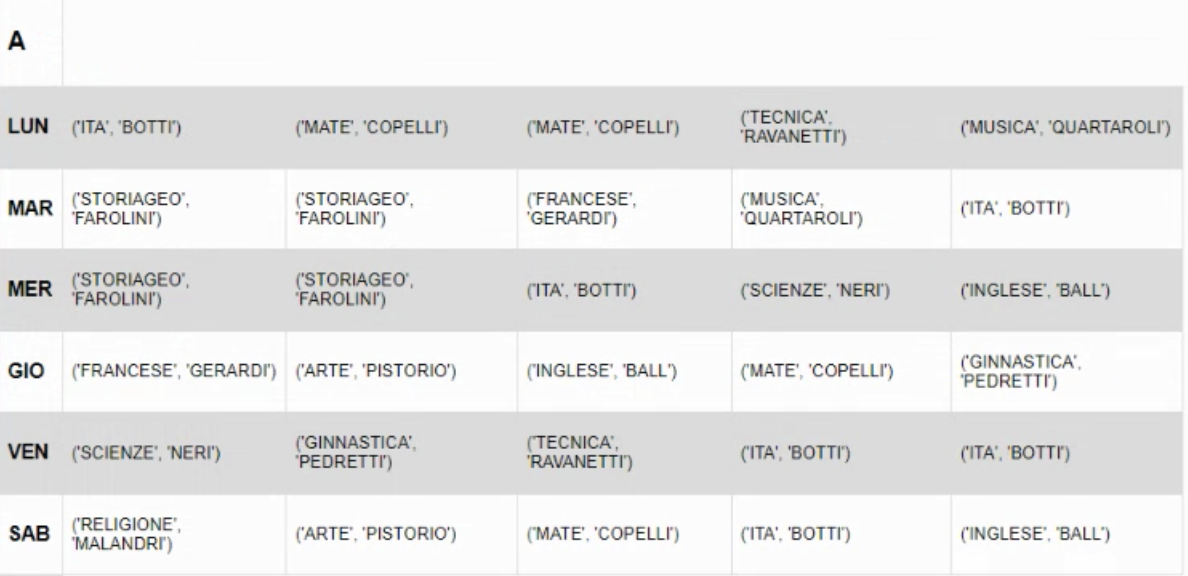
\includegraphics[width=\columnwidth]{Classe A 2.png}
  \end{center}
  \caption[Risultato AMPL]{Orario proposto dall'algoritmo per la classe A}
  \label{fig:Risultato AMPL A_2}
\end{figure}

\begin{figure}[H]
  \begin{center}
  \advance\leftskip-1cm
    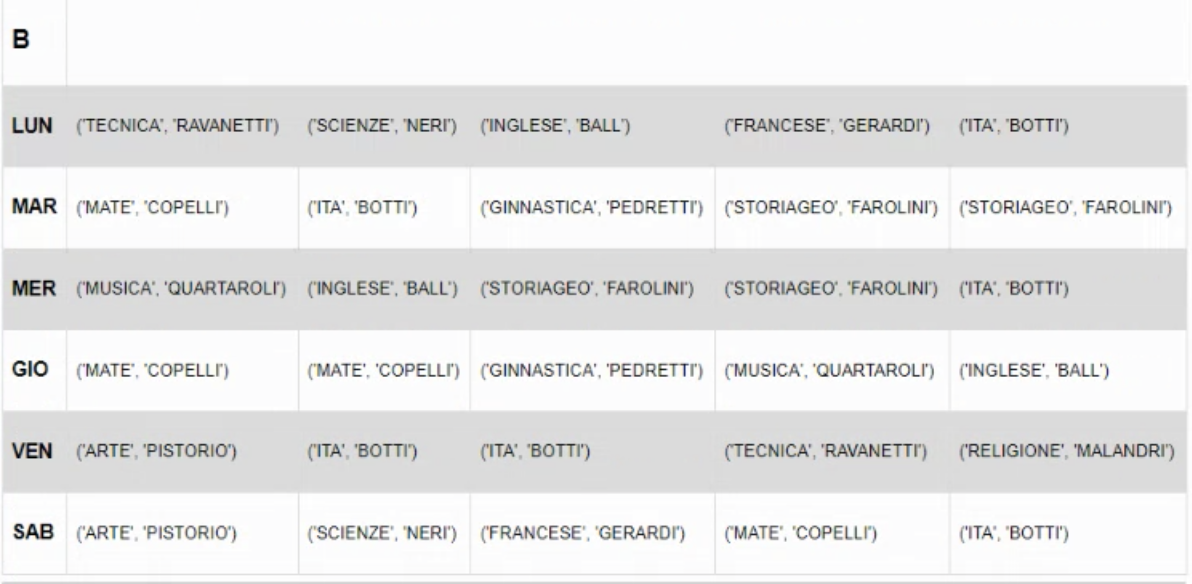
\includegraphics[width=\columnwidth]{Classe B 2.png}
  \end{center}
  \caption[Risultato AMPL]{Orario proposto dall'algoritmo per la classe B}
  \label{fig:Risultato AMPL B_2}
\end{figure}


\begin{figure}[H]
  \begin{center}
  \advance\leftskip-1cm
    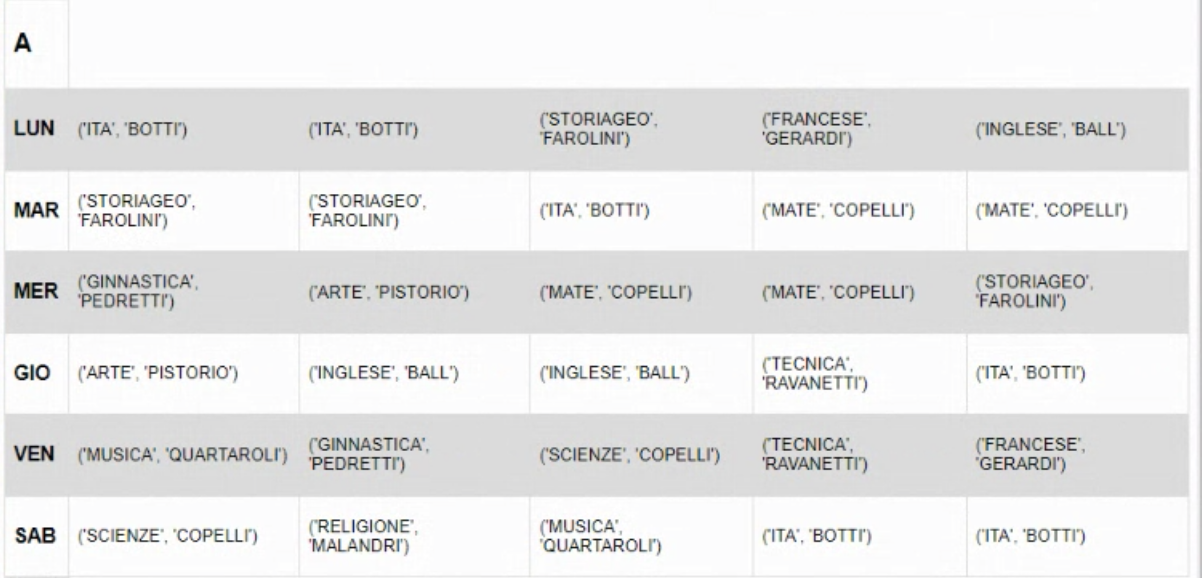
\includegraphics[width=\columnwidth]{Classe A 3.png}
  \end{center}
  \caption[Risultato AMPL]{Orario proposto dall'algoritmo per la classe A, nell'istanza con tre sezioni.}
  \label{fig:Risultato AMPL A_3}
\end{figure}

\begin{figure}[H]
  \begin{center}
  \advance\leftskip-1cm
    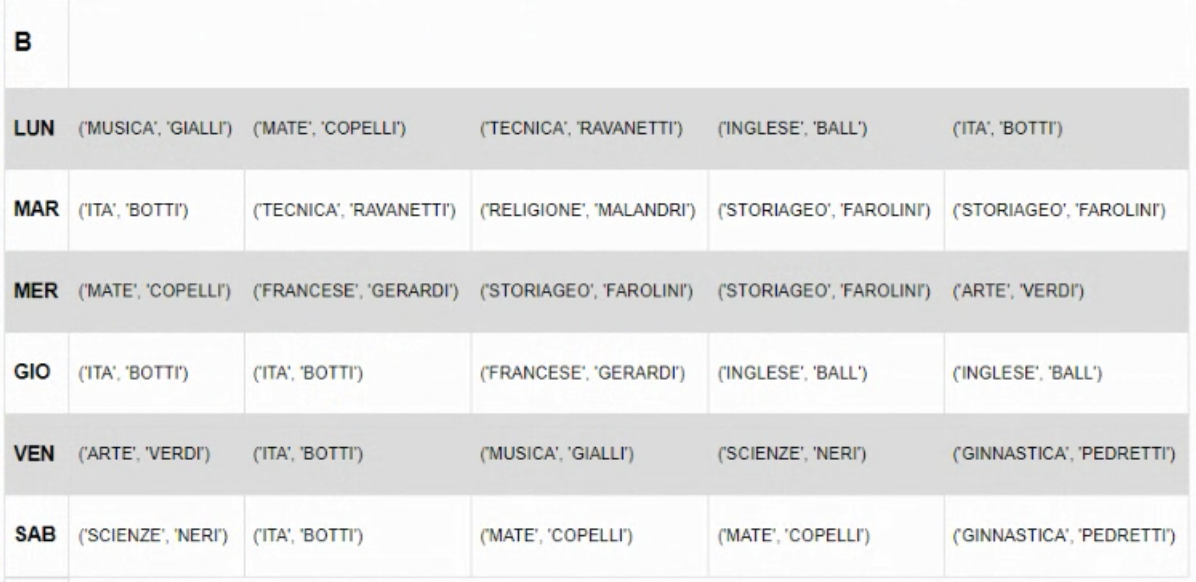
\includegraphics[width=\columnwidth]{Classe B 3.png}
  \end{center}
  \caption[Risultato AMPL]{Orario proposto dall'algoritmo per la classe B, nell'istanza con tre sezioni.}
  \label{fig:Risultato AMPL B_3}
\end{figure}

\begin{figure}[H]
  \begin{center}
  \advance\leftskip-1cm
    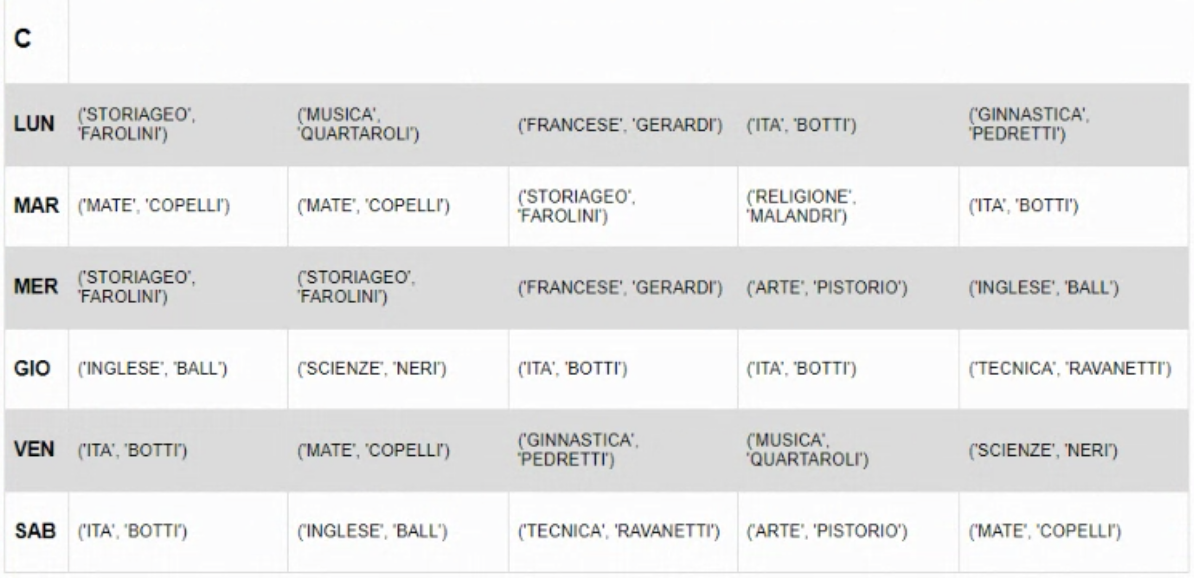
\includegraphics[width=\columnwidth]{Classe C 3.png}
  \end{center}
  \caption[Risultato AMPL]{Orario proposto dall'algoritmo per la classe C, nell'istanza con tre sezioni.}
  \label{fig:Risultato AMPL C_3}
\end{figure}




\section{Conclusioni}
Analizzando i risultati sopra riportati si nota come alcune delle richieste avanzate dai professori su giorni ed ore libere non siano soddisfatte. E' il caso, ad esempio, della richiesta fatta da Botti, nella seconda istanza del problema: Botti richiedeva l'indisponibilità al sabato alla seconda ora, ma l'algoritmo lo assegna alla sezione C, figura \ref{fig:Risultato AMPL C_3}. Allo stesso modo, sono presenti ore buche tra una lezione ed un'altra per alcuni professori, come sempre per Botti nella prima istanza, che ha lezione alla prima ed alla quinta ora. Per sicurezza, si è provato a convertire gli obiettivi in vincoli ad uno ad uno (quindi l'obiettivo di non lavorare nelle ore libere si traduceva in un \textbf{obbligo} di non lavorare nelle ore libere) e l'algoritmo ha prontamente modificato l'orario rispettando così i nuovi vincoli. Questo comporta il corretto funzionamento di ognuno degli obiettivi imposti. Di conseguenza, il modello elaborato, proposto come soluzione del problema di partenza, assume il comportamento previsto. Inoltre, ovviamente, nel caso in cui si proponesse un'istanza oggettivamente irrealizzabile, l'algoritmo proporrebbe un risultato nullo. E' il caso in cui si avessero 5 sezioni ed un solo professore abilitato ad insegnare italiano. Infatti, 5 sezioni comportano un totale di $5*6=30$ ore settimanali di italiano, ma il vincolo sul numero di giorni lavorativi (pari a 5) impone un massimo di $5*5=25$ ore settimanali per ogni professore. Pertanto l'istanza così descritta risulta essere infattibile, come vediamo riportato: 

\begin{minted}[bgcolor=lightGray]{AMPL}
ampl: option solver gurobi;
ampl: include 'C:\Users\lorenzo\assegnamento.run';
Gurobi 9.5.1: infeasible
800 simplex iterations
1 branch-and-cut nodes
No basis.
No primal variables returned.
\end{minted}


\section{Note}
E' possibile trovare tutti i codici dell'algoritmo al seguente \href{https://github.com/FilippoBotti/RicercaOperativa}{link}.
E' inoltre possibile replicare il risultato proposto in forma tabellare sopra presentato, attraverso l'uso dell'estensione di AMPL per il linguaggio Python (i codici sono sempre nella repository linkata) e il modulo Flask, sempre per Python.
\\I nomi dei professori corrispondono a nomi di professori avuti alle scuole medie.


\end{document}




